\section{Příklad 1}
% Jako parametr zadejte skupinu (A-H)
\prvniZadani{H}

Nejdříve si vypočítáme $U_{12}$:
$$U_{12} = U_1 + U_2 = 135 + 80 = 215 V$$

    \begin{figure}[htb]
    \centering
    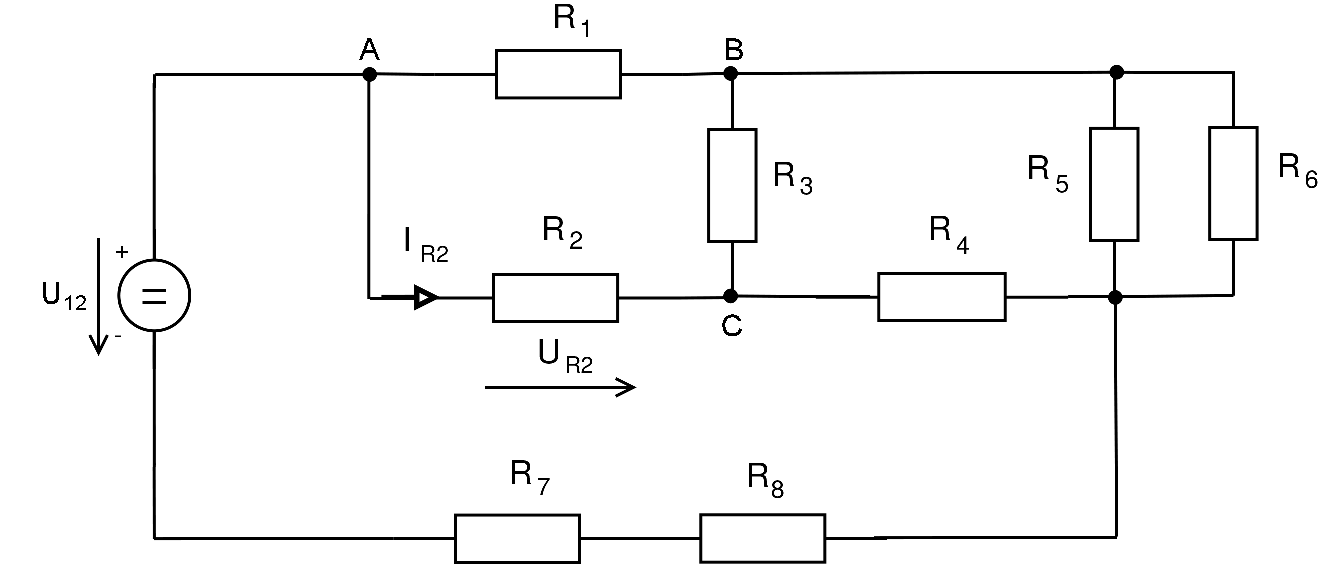
\includegraphics[scale=0.5,keepaspectratio]{sablona/fig/Pr1_Zdroje_oznaceni.pdf} \\
    \caption{Sločení zdrojů a označení uzlů}
    \end{figure}

\newpage

Převedeme trojúhelník na hvězdu: 
    \begin{figure}[htb]
    \centering
    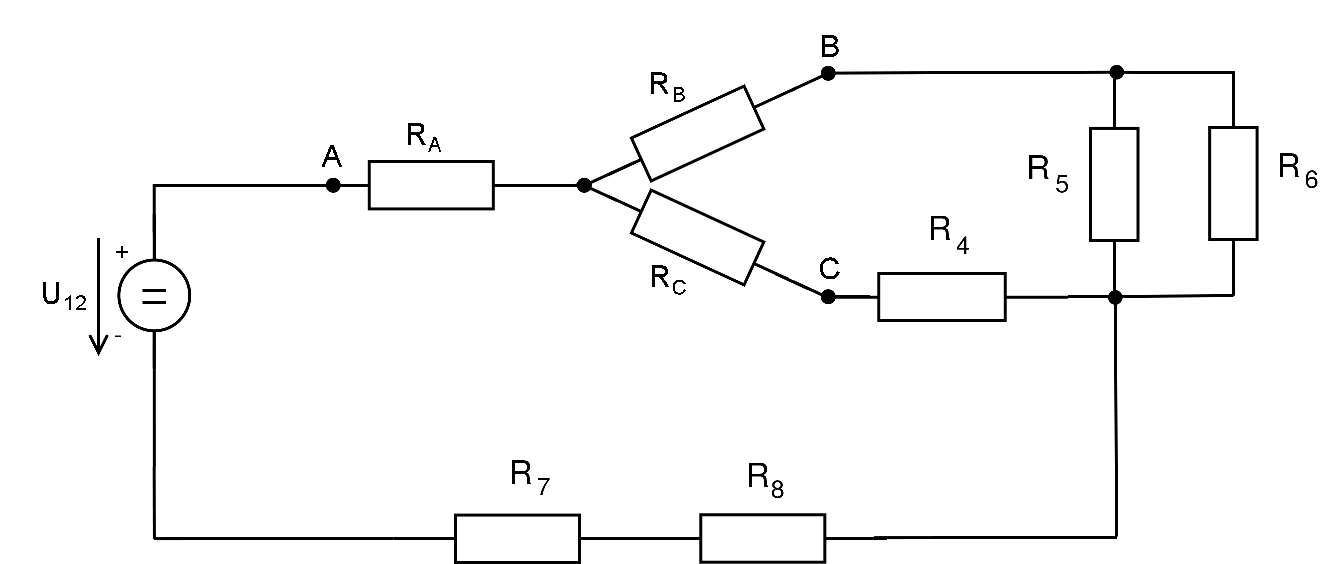
\includegraphics[scale=0.5,keepaspectratio]{sablona/fig/Pr1_Hvezda.pdf} \\
    \caption{Zapojení hvězda}
    \end{figure}

Vypočítáme odpory $R_A$, $R_B$, $R_C$:
$$R_A = \frac{R_1*R_2}{R_1 + R_2 + R_3} = \frac{680*600}{680+600+260} = 264,9350649\Omega$$
$$R_B = \frac{R_1*R_3}{R_1 + R_2 + R_3} = \frac{680*260}{680+600+260} = 114,8051948\Omega$$
$$R_C = \frac{R_2*R_3}{R_1 + R_2 + R_3} = \frac{600*260}{680+600+260} = 101,2987013\Omega$$
\newline

Vypočítáme si odpor $R_{56}$ a $R_{78}$:
$$R_{56} = \frac{R_5*R_6}{R_5+R_6} = \frac{575*870}{575+870} = 346,1937716\Omega$$
$$R_{78} = R_7 + R_8 = 355 + 265 = 620\Omega$$
    \begin{figure}[htb]
    \centering
    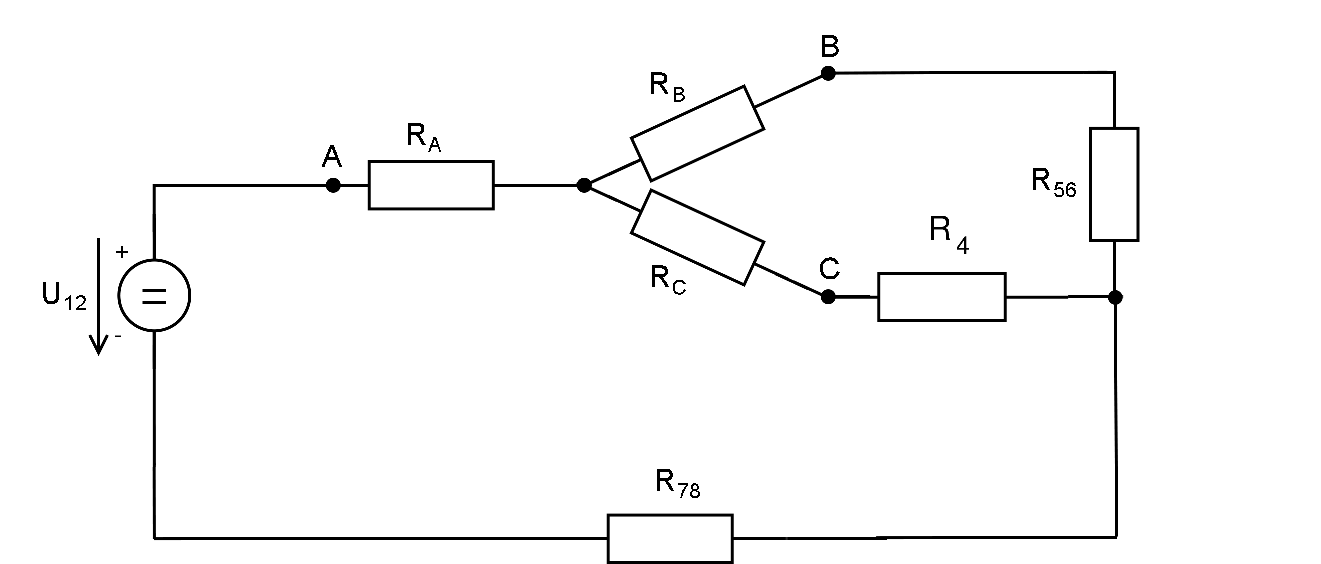
\includegraphics[scale=0.5,keepaspectratio]{sablona/fig/Pr1_urpava_REZ.pdf} \\
    \caption{Sečtení rezistorů $R_5$, $R_6$ a $R_7$, $R_8$}
    \end{figure}

\newpage

Vypočítáme si odpor $R_{C4}$ a $R_{B56}$:
$$R_{C4} = R_C + R_4 = 101,2987013 + 310 = 411,2987013\Omega$$
$$R_{B56} = R_B + R_{56} = 114,8051948 + 346,1937716 = 460,9989664\Omega$$
    \begin{figure}[htb]
    \centering
    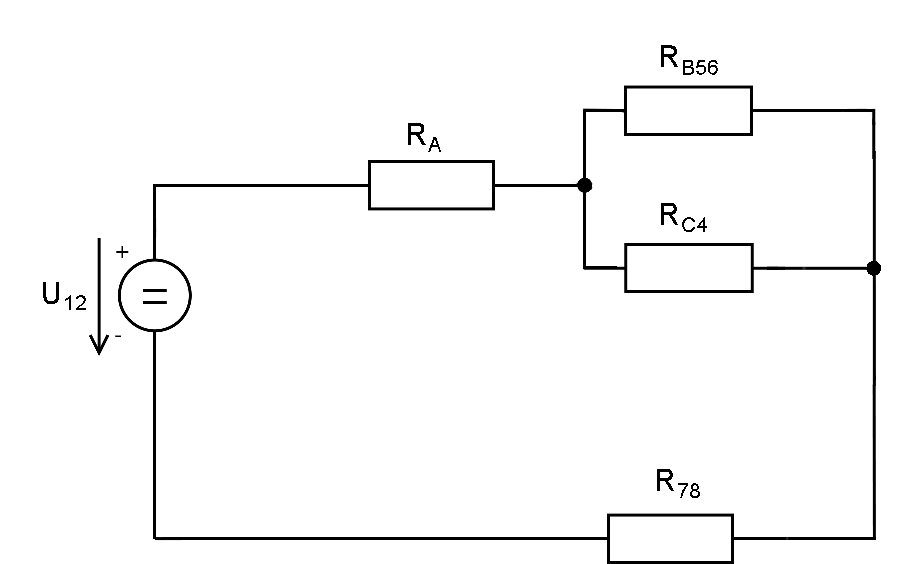
\includegraphics[scale=0.5,keepaspectratio]{sablona/fig/Pr1_Rezistory_BezHvezdy.pdf} \\
    \caption{Sečtení rezistorů $R_B$, $R_{56}$ a $R_C$, $R_4$}
    \end{figure}

Vypočítáme si odpor $R_{BC456}$:
$$R_{BC456} = \frac{R_{B56}*R_{C4}}{R_{B56}+R_{C4}} = \frac{460,9989664*411,2987013}{460,9989664+411,2987013} = 217,366483\Omega$$
    \begin{figure}[htb]
    \centering
    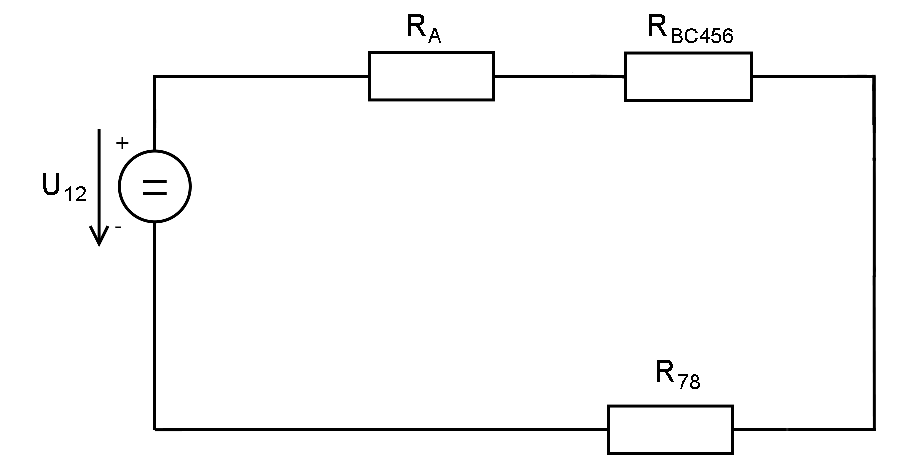
\includegraphics[scale=0.5,keepaspectratio]{sablona/fig/Pr1_RezistoryBezUzlu.pdf} \\
    \caption{Sečtení rezistorů $R_{B56}$ a $R_C4$}
    \end{figure}

Vypočítáme celkový odpor R:
$$R = R_A + R_{BC456} + R_{78} = 264,9350649 + 217,366483 + 620 = 1102,301548\Omega$$
    \begin{figure}[htb]
    \centering
    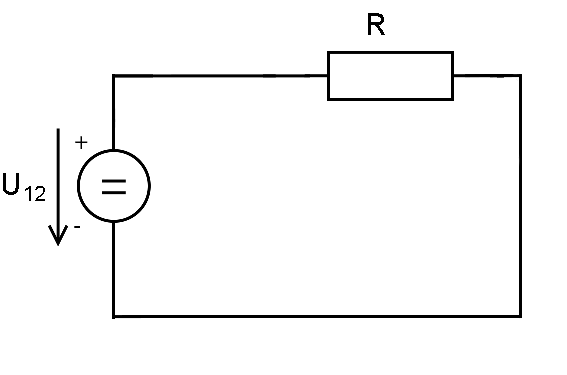
\includegraphics[scale=0.5,keepaspectratio]{sablona/fig/Pr1_CelkovyOdpor.pdf} \\
    \caption{Sečtení rezistorů $R_A$ a $R_{BC456}$ a $R_{78}$}
    \end{figure}

Za pomoci Ohmova zákona vypočítáme celkový proud obvodu:
$$I = \frac{U}{R} = \frac{215}{1102,301548} = 0,1950464466A$$
\newline

Vypočítáme $U_{R_A}$:
$$U_{R_A} = I * R_A = 0,1950464466 * 264,9350649 = 51,67464299V$$
\newline

Vypočítáme $U_{R_A}$:
$$U_{R_{BC456}} = I * R_{BC456} = 0,1950464466 * 217,366483 = 42,39656012V$$
\newline

Vypočítáme $I_{R_{B56}}$:
$$I_{R_{B56}} = \frac{U_{R_{BC456}}}{R_{B56}} = \frac{42,39656012}{460,9989664} = 0,09196671405A$$
\newline

Vypočítáme $I_{R_{C4}}$ a $U_{R_C}$:
$$I_{R_{C4}} = \frac{U_{R_{BC456}}}{R_{C4}} = \frac{42,39656012}{411,2987013} = 0,1030797325A$$
$$U_{R_C} = I{R_{C4}} * R_C = 0,1030797325 * 101,2987013 = 10,44184304$$
\newline

Teď už jsme schopni dopočítat $U_{R_2}$ a $I_{R2}$:
$$U_{R_2} = U_{R_A} + U_{R_C} = 51,67464299 + 10,44184304 = \mathbf{62,11648603V}$$
$$I_{R_2} = \frac{U_{R_2}}{R_2} = \frac{62,11648603}{600} = \mathbf{0,1035274767A}$$
